% ---------------------------------------------------------------------------
% R30/S12: dead-looking segment, suspected short at the output node (OS) to FS,
% and the implemented "2 of 3 CCDs" mitigation.
% Sources: "R30/S12 Issue" slides (meeting 2025-04-08); S. Marshall, NTP for
% implemented solution to running 2 of 3 CCDs, 2025-06-19; CCS logs of
% 2025-04-07 and 2025-06-03; trending of the 2025-06-25 back-bias ramp;
% A. Snyder, UCD report; #lsstcam Slack discussion (C. Lage, Y. Utsumi,
% S. Herrmann, S. Marshall, C. Juramy, G. Thayer, A. Snyder).
% Figures: fig_focalplane.pdf   (CTN-001 Fig. 1, R30/S12 boxes added here;
%                                built by fig_focalplane_build.tex)
%          fig_ccd250_pins.pdf  (drawn here, by fig_ccd250_pins.tex)
%          fig_output_lage.pdf  (C. Lage's LTspice schematic, cropped)
% ---------------------------------------------------------------------------

\subsubsection{R30/S12: dead-looking segment and suspected short}
\label{sec:r30s12}

On the e2v CCD S12 of raft R30 (RTM-012), read out by Reb1, the channel Seg17
reads essentially zero current and delivers no usable signal, and raising the
output drain (OD) of that REB towards its nominal value trips the
over-current protection within about 100~ms. Three such trips were recorded
(\S\ref{sec:r30s12-trips}).

The REB measures each channel's current on the low side of its current
source, so a channel whose output node is held near 0~V reads $\simeq0$~mA.
The discussion of these data points to a short between the output node of the
affected channel (OS, the source of the output transistor) and FS, which is at
or near ground; a short involving OD was also raised as plausible, given the
large total OD current seen when OD is raised. An ITL sensor showed the same
signature about five years ago and was concluded to have a
short.\footnote{\emph{Summary on dead looking channels}, LSSTCam Confluence,
\url{https://confluence.slac.stanford.edu/spaces/LSSTCAM/pages/240279059/Summary+on+dead+looking+channels}.}

REB5 has no per-channel OD control, so the fault is isolated at the level of
the CCD instead: S12 is powered only partially, with its OD setpoint reduced
to 0.15 (measured ODV $\simeq2$~V), and S10 and S11 on the same REB operate
normally. This required a special REB firmware build and a set of CCS
configuration and test changes, validated at UC Davis
(\S\ref{sec:r30s12-solution}). The cost is one CCD out of the three on Reb1.

\paragraph{Location and pin arrangement.}
\label{sec:r30s12-location}

\begin{figure}[htbp]
  \centering
  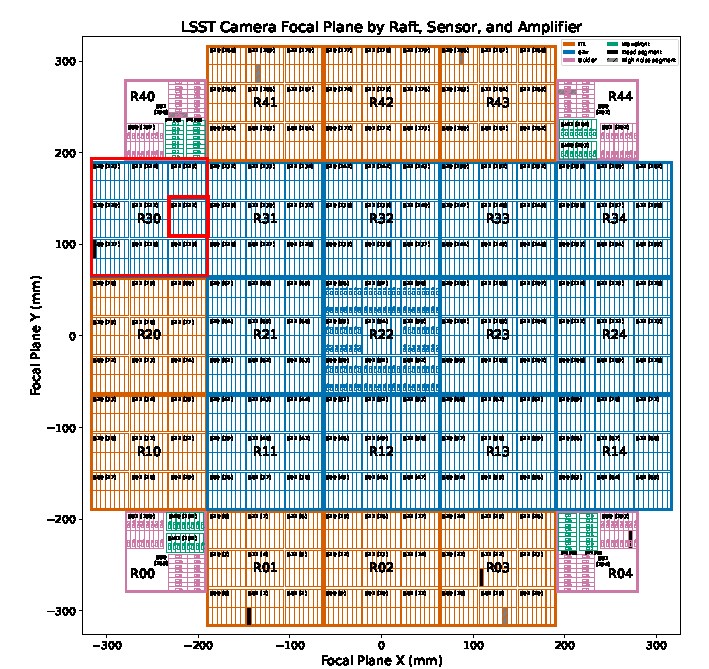
\includegraphics[width=0.85\textwidth]{r30s12/fig_focalplane.pdf}
  \caption{LSSTCam focal plane layout, after \citet[Fig.~1]{CTN-001}. The large
    red box marks R30 = RTM-012 and the small box indicates the sensor S12.}
  \label{fig:r30s12-focalplane}
\end{figure}

\begin{figure}[htbp]
  \centering
  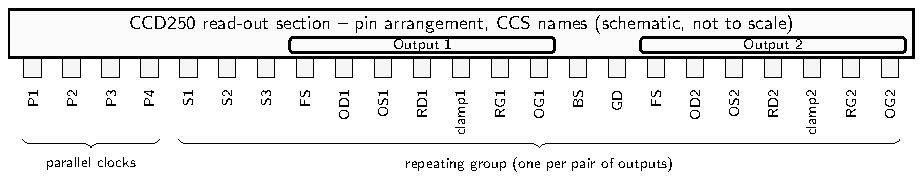
\includegraphics[width=\textwidth]{r30s12/fig_ccd250_pins.pdf}
  \caption{Pin arrangement of the CCD250 read-out section in CCS names, drawn
    after the pin order given in the CCD250 Design Report \citep{e2v:ccd250}.
    The names are explained in the text.}
  \label{fig:ccd250-pinout}
\end{figure}

R30 is an e2v raft; Reb1 reads S10, S11 and S12
(Fig.~\ref{fig:r30s12-focalplane}). The read-out section of the CCD250 is
organised in a repeating group; in CCS names the pin order is
\texttt{S1 S2 S3 FS OD1 OS1 RD1 clamp1 RG1 OG1 BS GD FS OD2 OS2 RD2 clamp2
RG2 OG2}, preceded by the parallel clocks \texttt{P1}--\texttt{P4}
(Fig.~\ref{fig:ccd250-pinout}). Here P1--P4 are the parallel (image) clocks
and S1--S3 the serial clocks; OD is the output drain, OS the output amplifier
source, RD the reset transistor drain and RG the reset transistor gate; OG is
a DC bias at the end of the serial register, ahead of the sense node and the
reset transistor; FS and BS are the front and back substrate and GD the guard
diode. The clamp gate (\emph{Reset~2} in
Fig.~\ref{fig:output-stage}) is connected to P4.

\paragraph{The turn-on sequence.}
\label{sec:r30s12-sequence}

\texttt{powerCCDsOn} sequences the biases RD, OD, GD, OG. RD, GD and OG are
written to the DAC, applied, and sampled for $\sim160$~ms before the currents
and voltages are checked against the configured limits; a limit that is
exceeded ends the sequence with an exception. OD is stepped instead: first to
15~V with a $\sim100$~ms check, then to the configured value. Bias voltages
are read every 5.3~ms (\texttt{readSlowAdcs()}) and parent currents every
33~ms (\texttt{readPowerAdcs()}), each set carrying one timestamp taken at the
start of the call. Each trip is therefore documented by only a few samples,
and the voltage at which the current peaked is loosely constrained.

\paragraph{Three over-current trips.}
\label{sec:r30s12-trips}

Three attempts to power on R30/Reb1 failed with an OD over-current condition
(Table~\ref{tab:r30s12-events}). The log of the first reads

\begin{quote}\small\ttfamily
[2025-04-07T20:51:27.238+0000] SEVERE: , R30/Reb1/Bias2 OD2 Overcurrent
measured on ODI: 0.213 > 0.082 (odIMax (A))
\end{quote}

\noindent followed by \texttt{powerCCDsOn() FAILED for R30/Reb1} and, 0.8~s
later, an automatic \texttt{powerCCDsOff()}. In each case the DAC was set back
to zero immediately, returning OD to 0~V within $100$--$140$~ms of the step.

\begin{table}[htbp]
  \centering
  \caption{The three failed power-on attempts. \texttt{ODV} is
    \texttt{focal-plane/R30/Reb1/S12/ODV} and \texttt{ODI} is
    \texttt{focal-plane/R30/Reb1/ODI}, the REB-level total. The threshold
    \texttt{odIMax} is 82~mA in the log message and quoted as 83~mA in
    \citet{marshall:ntp}. $\Delta t$ is the interval between the step and the
    sample that exceeded it.}
  \label{tab:r30s12-events}
  \begin{tabular}{lccccc}
    \hline
    Event & Time (UTC) & OD step & last \texttt{ODV} & peak \texttt{ODI}
          & $\Delta t$ \\
    \hline
    1 & 2025-04-07T20:51:27 & $0 \rightarrow 15$~V    & 14.94~V & 213.1~mA & $\sim140$~ms \\
    2 & 2025-04-07T20:54:32 & $15 \rightarrow 22.3$~V & 22.27~V & 220.6~mA & $\sim100$~ms \\
    3 & 2025-06-03T19:09:08 & $15 \rightarrow 22.3$~V & 22.3~V  & $>83$~mA & $\sim100$~ms \\
    \hline
  \end{tabular}
\end{table}

Only three current samples exist per April event, and in the first the last
voltage sample before the 213~mA reading was 14.9~V. Taking the excess current
to flow through a resistive path, $R_{\mathrm{short}} = V/\Delta I$ gives
%
\begin{equation}
  R_1 \simeq 125~\Omega, \qquad R_2 \simeq 208~\Omega
  \label{eq:rshort}
\end{equation}
%
for the two events \citep{marshall:ntp}. The June peak lies just above the
threshold, well below the April peaks.

\paragraph{Quiescent behaviour.}

Trending of \texttt{focal-plane/R30/Reb1/ODI} through the afternoon of
2025-04-07, during telescope slews and before the first trip, shows a flat
$\simeq69.6$~mA: the monitoring carried no precursor of the fault.

\paragraph{Vacuum and temperature response.}

Each April trip is accompanied by a rise of \texttt{vacuum/Cryo/CryoVac} from
$1.31\times10^{-7}$ to $1.47\times10^{-7}$~Torr, decaying over a few minutes,
and by a $\sim0.25$~$^\circ$C excursion of
\texttt{focal-plane/R30/Reb1/Temp9}; the ion-pump currents
(\texttt{vacuum/Cryo/CIP1\_I} to \texttt{CIP6\_I}) and the cold-plate RTDs do
not change significantly. This indicates localised power dissipation at the
fault site.

\paragraph{Interpretation.}
\label{sec:r30s12-cause}

\begin{figure}[htbp]
  \centering
  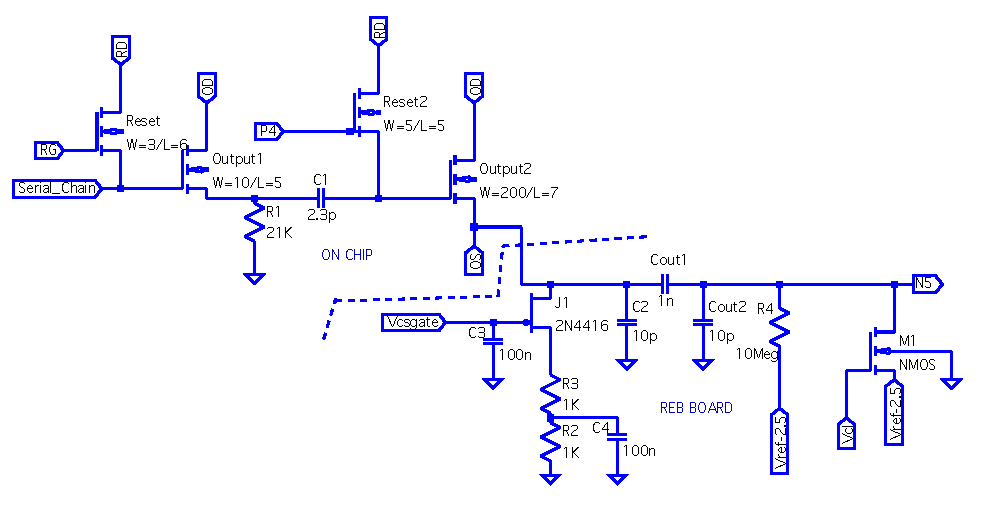
\includegraphics[width=\textwidth]{r30s12/fig_output_lage.pdf}
  \caption{The e2v output stage and the first stage of the REB circuit, drawn
    by C. Lage \citep{lage:circuit}. The two on-chip source followers (\emph{Output1}, \emph{Output2}) are
    coupled through C1, with the clamp \emph{Reset~2} on that node driven by
    P4; \emph{Output2} drives the OS pin into the current source J1 on the
    REB, whose return to ground through R3 and R2 carries the per-segment
    current monitor. The suspected short is from the OS node to ground.}
  \label{fig:output-stage}
\end{figure}

A shorted segment reading zero current follows from where the currents are
measured (Fig.~\ref{fig:output-stage}). Each segment current is monitored on
the low side of that segment's current source, its return to ground, whereas
the OD current is measured only as a total, for the CCD's OD supply as a
whole. If the output node of a segment, the source of the output transistor,
is held at 0~V by a short to ground, the current source cannot force its
current and the segment monitor reads 0~mA. An open connection reads the same,
since a current source cannot impose a current into an unterminated node
either.

\texttt{Bias2}/\texttt{OD2} in the log message is the OD supply of S12, and
its current is measured for that supply as a whole, so a short anywhere in the
CCD raises it: the over-current localises the fault to S12 but does not
identify the segment. It is the zero reading on Seg17 that points to that
segment.

It was also noted in the discussion that the shorted node need not be at
ground potential but could sit a couple of diode drops above it; the current
source still needs some positive compliance voltage, so the effect would be
the same, through a diode rather than through a resistance.

The $\simeq2$~V that ODV still reads with the OD DAC at essentially zero has
its own explanation, and is not evidence about the CCD. The current source on
the REB is not turned off in that state: its gate DAC (\texttt{csGate}) passes
$\simeq1$~mA at a setting of 0 and $\simeq3$~mA at 255, and the focal plane is
already run at 0, while shutting the 2N4416 JFET off would take about
$-3$~V on its gate, which the REB cannot supply. That current flows through
the on-chip output transistor and the two $1$~k$\Omega$ resistors in the JFET
source, developing $\simeq2$~V at that node, which pulls up OS and with it OD.
The same floor is measured on a healthy CCD at UC Davis, 2.01~V with the
back-bias off
(Table~\ref{tab:ucd}). The question raised at the time was whether current
could flow from the REB circuit into the OS side of the CCD and across the
short to ground; at $\simeq1$~mA and $\simeq2$~V it was judged small enough to
proceed.

\subsubsection{R30/S12: running two of the three CCDs on Reb1}
\label{sec:r30s12-solution}

\paragraph{Concept.}

S12 is powered only partially, leaving its ODV at $\simeq0$
\citep{marshall:ntp}. The OD setpoint is 0.15, for which ODV measures
$\simeq2$~V and decreases further as the back-bias is applied. RD and GD stay
nominal, so the CCD remains protected when hvbias is turned on, while the OD
current stays far below \texttt{odIMax}. S10 and S11 are powered normally;
S12 produces no signal.

\paragraph{Firmware and CCS changes.}

The REB firmware protects against writing GD, OD or RD below hard-coded
thresholds and prevents closing the back-bias switch while any of them is
below its threshold, and the CCS power-on and power-state methods both reject
an OD of $\simeq0$~V. The changes are:

\begin{itemize}
  \item \emph{REB firmware}, version \texttt{0x31395011} (Table~\ref{tab:science_reb_fw_en}),
        backward compatible and with the default behaviour unchanged. It makes all bias thresholds readable by CCS
        (registers \texttt{0x401100}--\texttt{0x401124}) and adds a
        per-sensor sequencer override register
        (\texttt{0x400010}--\texttt{0x400012}) that drives the sensor lines
        with static values instead of the sequencer, without stopping
        digitisation, which would otherwise break the CCS data decoding.
  \item \emph{A dedicated instance of that firmware for R30/Reb1}, with the
        OD threshold set to zero. It is otherwise identical and reports the
        same version number, so it is identified by \texttt{R30\_Reb1}
        appended to the design name, which appears in the bitfile header and
        filename and is checked before loading to EEPROM so that this
        instance cannot be loaded onto another REB. The nominal
        \texttt{0x31395011} build was proposed for all REBs after testing on
        TS8, so that the threshold read-back is not available on one REB
        only.
  \item \emph{CCS}: the power-on and power-state tests were modified to accept
        ODV $\simeq0$. The hvbias threshold test passes only with the special
        firmware installed; the board-level current test needs a smaller
        \texttt{odiAmin}; and with an OD setpoint in $0.1$--$1.0$ the OD
        voltage passes both the ON and the OFF test, so the CCD state follows
        from the aggregate result for OD, GD, RD and OG. In total
        \texttt{odTol}, \texttt{odZeroErr}, \texttt{odP} and
        \texttt{odiAmin} were re-valued.
  \item \emph{Configuration}: the OD lower limit of the S12 bias block was
        changed in \texttt{camera-dp80.properties},

        \begin{quote}\small\ttfamily
        -~R30/Reb1/Bias2/odMin = 21.30 \\
        +~R30/Reb1/Bias2/odMin = 0.0
        \end{quote}

        \noindent leaving \texttt{gdMin}, \texttt{odMax}, \texttt{ogMax}
        and \texttt{ogMin} for that block unchanged, and the tolerances were
        widened in \texttt{camera.properties},

        \begin{quote}\small\ttfamily
        -~R30/Reb1/odiAmin = 0.023 \\
        +~R30/Reb1/odiAmin = 0.018 \\
        -~R30/Reb1/Bias2/gdTol = 0.25 \\
        +~R30/Reb1/Bias2/gdTol = 0.90 \\
        -~R30/Reb1/Bias2/odTol = 0.1 \\
        +~R30/Reb1/Bias2/odTol = 2.1 \\
        -~R30/Reb1/Bias2/odZeroErr = 0.2 \\
        +~R30/Reb1/Bias2/odZeroErr = 2.2
        \end{quote}

        \noindent with \texttt{odIMax} for that block left at 0.082.
\end{itemize}

\paragraph{Validation at UC Davis.}
\label{sec:r30s12-ucd}

The changes were exercised on the e2v beam simulator at UC Davis, with a
single CCD, one science REB and non-LSST power supplies
\citep{ucd:vodzero}. The OD setpoint was set to 0.151~V in the CCS properties
file, the CCD powered on while ODI, ODV and the back-bias voltage and current
were measured, a series of bias images taken with those monitored, and the
back-bias then incremented
(Table~\ref{tab:ucd}). The CCS properties changed to let that CCD
(\texttt{R21/Reb0/Bias1}) run with OD off were

\begin{quote}\small\ttfamily
R21/Reb0/odiAmin=0.005 \\
R21/Reb0/Bias1/gdTol=0.7 \\
R21/Reb0/Bias1/odTol=2.1 \\
R21/Reb0/Bias1/odZeroErr=2.2 \\
R21/Reb0/Bias1/odP=0.15 \\
R21/Reb0/Bias1/odMin=0.0
\end{quote}

\noindent in the \texttt{RaftsPower}, \texttt{Rafts} and
\texttt{RaftsLimits} properties files respectively, with
\texttt{csGate}$\,=0.0$. The OD setpoint is quoted as 0.151~V in
\citet{ucd:vodzero}.

\begin{table}[htbp]
  \centering
  \caption{UC Davis measurements with the OD setpoint at 0.15
    \citep{ucd:vodzero}. $V_{\mathrm{bs}}$ and $I_{\mathrm{bs}}$ are the
    back-bias voltage and current, commanded and read as indicated; the report
    labels them BSS, VSS and ISS. Blank entries were not recorded.}
  \label{tab:ucd}
  \begin{tabular}{cccccc}
    \hline
    $V_{\mathrm{bs}}$ cmd (V) & $V_{\mathrm{bs}}$ read (V) &
    $I_{\mathrm{bs}}$ (mA) & ODV (V) & ODI (mA) & Seg00 $I$ (mA) \\
    \hline
     0 &  0.00 & 0.0 & 2.01 & 27.7 & \\
     5 &  5.01 & 0.1 & 1.83 &      & 0.8   \\
    10 & 10.01 & 0.0 & 1.64 & 25.9 & 0.737 \\
    20 & 20.02 & 0.1 & 1.32 & 23.9 & 0.61  \\
    30 & 30.03 & 0.1 & 1.02 & 21.8 & 0.483 \\
    40 & 40.02 & 0.1 & 0.73 & 19.8 & 0.358 \\
    50 & 50.02 & 0.1 & 0.46 & 17.8 & 0.238 \\
    \hline
  \end{tabular}
\end{table}

The minimum ODV with the back-bias off is 2.01~V, and ODV, ODI and the
per-segment current all decrease as $V_{\mathrm{bs}}$ is raised. The read
$V_{\mathrm{bs}}$ shows no variation during bias readout and
$I_{\mathrm{bs}}$ fluctuates between 0.0 and 0.1~mA, at the resolution of the
supply. Bias images taken in this mode resemble bias images taken with the CCD
powered off. For reference, the same CCD at nominal dp80 voltages draws an ODI
of 34.6~mA, both with the back-bias off and at 50~V, and 9.4~mA with the CCD
powered off; these were measured to set \texttt{odiAmin} for R30/Reb1, which
was lowered from 0.023 to 0.018. The report notes that the changes of ODV and ODI with the
back-bias on will require further modification of the CCS limits.

\paragraph{Behaviour on the summit.}
\label{sec:r30s12-ramp}

The configuration was exercised during the manual back-bias ramp of
2025-06-25, 18:45--19:30~UTC, trended with

\begin{quote}\small\ttfamily
trender.py --overlayregex --start '2025/6/25 18:45:00' --plot --dur 1h \\
'focal-plane/R30/Reb1/ODI' 'focal-plane/R30/Reb1/S12/Seg1[57]/I' \\
'rebpower/R30/Reb1/hvbias/.*' 'vacuum/Cryo/CryoVac'
\end{quote}

\noindent As
\texttt{rebpower/R30/Reb1/hvbias/VbefSwch} was stepped from 0 to 50~V,
\texttt{focal-plane/R30/Reb1/ODI} fell monotonically from 66.4 to 55.3~mA and
\texttt{.../S12/Seg15/I} from 0.83 to 0.29~mA, while \texttt{.../S12/Seg17/I}
stayed at the noise level ($\simeq0.02$~mA falling to $\simeq0$~mA);
\texttt{hvbias/IbefSwch} rose from 0 to 0.08~mA with the DAC going from
$\simeq1250$ to $\simeq1550$, and \texttt{vacuum/Cryo/CryoVac} was stable at
$7.4\times10^{-8}$~Torr. The currents therefore decrease with increasing
back-bias as at UC Davis, the ramp produced no vacuum or current excursion,
and Seg17 remained dead throughout.

\paragraph{Operational consequences.}

The configuration recovers two of the three CCDs on Reb1 and keeps the raft
protected during hvbias turn-on, at the price of S12. Two points follow from
how it is achieved: the special firmware must remain installed on this REB for
the hvbias threshold test to pass, and the relaxed parameters
(\texttt{odTol}, \texttt{odZeroErr}, \texttt{odP}, \texttt{odiAmin}) weaken,
for this REB, the tests meant to catch this class of fault. Both should be
tracked in configuration management. The mitigation has been in effect since
2025-06-25; the firmware \texttt{0x31395011} had been rolled out to the focal
plane before that date. S12 is not masked in the acquisition configuration, so
its frames are read out and written even though they carry no signal.

\paragraph{Outlook.}
\label{sec:r30s12-consequences}

\begin{itemize}
  \item Running this REB at nominal OD is not an option: the protection trips
        within about 100~ms, and each attempt deposits energy at the fault
        site.
  \item There is no in-situ repair path; reaching the fault would require
        breaking vacuum and disassembly.
  \item The granularity of the mitigation is set by the electronics, not by
        the fault: OD can only be lowered for a whole CCD, so a single
        shorted segment costs a sensor.
\end{itemize}
